\documentclass[11pt]{charter}

% El títulos de la memoria, se usa en la carátula y se puede usar el cualquier lugar del documento con el comando \ttitle
\titulo{Sistema de monitoreo en tiempo real para el adulto mayor} 

% Nombre del posgrado, se usa en la carátula y se puede usar el cualquier lugar del documento con el comando \degreename
\posgrado{Carrera de Especialización en Sistemas Embebidos} 
%\posgrado{Carrera de Especialización en Internet de las Cosas} 
%\posgrado{Carrera de Especialización en Intelegencia Artificial}
%\posgrado{Maestría en Sistemas Embebidos} 
%\posgrado{Maestría en Internet de las cosas}

% Tu nombre, se puede usar el cualquier lugar del documento con el comando \authorname
\autor{William's Ernesto Limonchi Sandoval} 

% El nombre del director y co-director, se puede usar el cualquier lugar del documento con el comando \supname y \cosupname y \pertesupname y \pertecosupname
\director{Lucas Dórdolo}
\pertenenciaDirector{pertenencia} 
% FIXME:NO IMPLEMENTADO EL CODIRECTOR ni su pertenencia
\codirector{} % si queda vacio no se deberíá incluir 
\pertenenciaCoDirector{}

% Nombre del cliente, quien va a aprobar los resultados del proyecto, se puede usar con el comando \clientename y \empclientename
\cliente{Javier Vasquez de Velasco}
\empresaCliente{Especialista Ferreyros}

% Nombre y pertenencia de los jurados, se pueden usar el cualquier lugar del documento con el comando \jurunoname, \jurdosname y \jurtresname y \perteunoname, \pertedosname y \pertetresname.
\juradoUno{Nombre y Apellido (1)}
\pertenenciaJurUno{pertenencia (1)} 
\juradoDos{Nombre y Apellido (2)}
\pertenenciaJurDos{pertenencia (2)}
\juradoTres{Nombre y Apellido (3)}
\pertenenciaJurTres{pertenencia (3)}
 
\fechaINICIO{13 de octubre de 2020}		%Fecha de inicio de la cursada de GdP \fechaInicioName
\fechaFINALPlanificacion{11 de diciembre de 2020} 	%Fecha de final de cursada de GdP
\fechaFINALTrabajo{22 de agosto de 2021}		%Fecha de defensa pública del trabajo final


\begin{document}

\maketitle
\thispagestyle{empty}
\pagebreak


\thispagestyle{empty}
{\setlength{\parskip}{0pt}
\tableofcontents{}
}
\pagebreak


\section{Registros de cambios}
\label{sec:registro}


\begin{table}[ht]
\label{tab:registro}
\centering
\begin{tabularx}{\linewidth}{@{}|c|X|c|@{}}
\hline
\rowcolor[HTML]{C0C0C0} 
Revisión & \multicolumn{1}{c|}{\cellcolor[HTML]{C0C0C0}Detalles de los cambios realizados} & Fecha      \\ \hline
1.0      & Creación del documento                                          & 23/10/2020 \\ \hline
1.1      & Presentación hasta el punto 6                                   & 06/11/2020 \\ \hline
1.2      & Correcciones de Practico 1                                      & 06/11/2020 \\ \hline
%1.2      & Otro ejemplo \newline
%		   Con texto partido \newline
%		   En varias líneas \newline
%		   A propósito                                                     & dd/mm/aaaa \\ \hline
\end{tabularx}
\end{table}

\pagebreak



\section{Acta de constitución del proyecto}
\label{sec:acta}

\begin{flushright}
Buenos Aires, \fechaInicioName
\end{flushright}

\vspace{2cm}

Por medio de la presente se acuerda con el Ing. \authorname\hspace{1px} que su Trabajo Final de la \degreename\hspace{1px} se titulará ``\ttitle'', consistirá esencialmente en observar la temperatura, nivel de saturación de oxígeno y detectar caída del adulto mayor en tiempo real, y tendrá un presupuesto preliminar estimado de 611 hs de trabajo con fecha de inicio \fechaInicioName\hspace{1px} y fecha de presentación pública \fechaFinalName.

Se adjunta a esta acta la planificación inicial.

\vfill

% Esta parte se construye sola con la información que hayan cargado en el preámbulo del documento y no debe modificarla
\begin{table}[ht]
\centering
\begin{tabular}{ccc}
\begin{tabular}[c]{@{}c@{}}Ariel Lutenberg \\ Director posgrado FIUBA\end{tabular} & \hspace{2cm} & \begin{tabular}[c]{@{}c@{}}\clientename \\ \empclientename \end{tabular} \vspace{2.5cm} \\ 
\multicolumn{3}{c}{\begin{tabular}[c]{@{}c@{}} \supname \\ Director del Trabajo Final\end{tabular}} \vspace{2.5cm} \\
%\begin{tabular}[c]{@{}c@{}}\jurunoname \\ Jurado del Trabajo Final\end{tabular}     &  & \begin{tabular}[c]{@{}c@{}}\jurdosname\\ Jurado del Trabajo Final\end{tabular}  \vspace{2.5cm}  \\
%\multicolumn{3}{c}{\begin{tabular}[c]{@{}c@{}} \jurtresname\\ Jurado del Trabajo Final\end{tabular}} \vspace{.5cm}                                                                     
\end{tabular}
\end{table}




\section{Descripción técnica-conceptual del proyecto a realizar}
\label{sec:descripcion}

\begin{consigna}{black}
El 30 de enero de 2020, la OMS declaró la epidemia de COVID-19, esta enfermedad respiratoria provoca mayor mortalidad en personas mayores de 60 años. Una medida que han adoptado todos los países ha sido el distanciamiento social lo que genera que las familias estén lejos de sus familiares más adultos, además de desconocer el estado de salud de sus seres queridos. 

El objetivo del sistema a desarrollar es conocer el nivel de temperatura, el nivel de saturación de oxígeno en la sangre y si adulto mayor ha sufrido alguna caída. El microcontrolador obtiene toda esta data mediante los diferentes sensores para luego procesar y almacenar la información en un memoria micro SD. Asimismo, esta información es transmitida mediante un módulo Wifi hacia una plataforma Web en la que el usuarios o los usuarios puedan observar la data obtenida. 

El presente proyecto se destaca especialmente por incorporar un sistema en tiempo real por lo que se monitorea y notifica, de presentarse alguna eventualidad, de la manera más rápida y óptima. 

En la Figura 1 se muestra el diagrama de bloques del sistema. Se observa el microcontrolador con cada uno de los sensores del sistema, así como  el módulo de alimentación que será una batería y por último, el Wifi que transmite la información hacía la página web.

\vspace{25px}

\begin{figure}[htpb]
\centering 
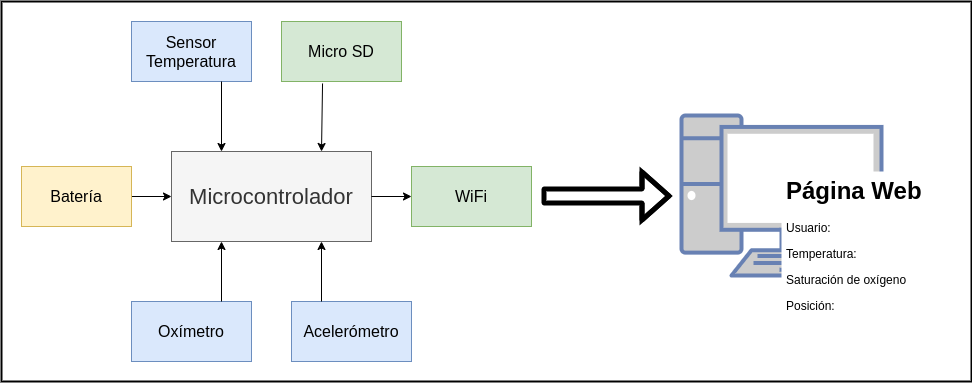
\includegraphics[width=1\textwidth]{./Figuras/diagBloques.png}
\caption{Diagrama en bloques del sistema}
\label{fig:diagBloques}
\end{figure}

\vspace{25px}

\end{consigna}


\section{Identificación y análisis de los interesados}
\label{sec:interesados}

\begin{consigna}{black} 
\vspace{-35px}
\begin{itemize}
\item Auspiciante: es riguroso y exigente con la rendición de gastos y en el desarrollo del proyecto en el tiempo establecido.
\item Cliente: Javier Vasquez de Velasco, interesado en el desarrollo del proyecto para utilizarlo en el monitoreo de su madre que padece de una enfermedad.
\end{itemize}

\begin{table}[ht]
%\caption{Identificación de los interesados}
%\label{tab:interesados}
\begin{tabularx}{\linewidth}{@{}|l|X|X|l|@{}}
\hline
\rowcolor[HTML]{000000} 
Rol           & Nombre y Apellido & Organización 	& Puesto 	\\ \hline
Auspiciante   & Williams Limonchi Falen & - 		& Mecánico	\\ \hline
Cliente       & \clientename     &\empclientename	& Ing. Mecánico	\\ \hline
Impulsor      & -                 & -              	& -       	\\ \hline
Responsable   & \authorname       & FIUBA        	& Alumno 	\\ \hline
Colaboradores & -                 & -             	& -       	\\ \hline
Orientador    & \supname	      & \pertesupname 	& Director	Trabajo final \\ \hline
Equipo        & - \newline 
				-          & -            	& -       	\\ \hline
Opositores    & Wok Solución      & -            	& -      	\\ \hline
Usuario final & Adultos mayores   & -              	& -      	\\ \hline
\end{tabularx}
\end{table}


\end{consigna}



\section{1. Propósito del proyecto}
\label{sec:proposito}

\begin{consigna}{black}
El propósito de este proyecto es desarrollar un prototipo de monitoreo en tiempo real de un adulto mayor. Este desarrollo permite visualizar el estado de temperatura, saturación de oxígeno y si el adulto mayor ha sufrido alguna caída. Además de notificar por si ocurre alguna eventualidad a los familiares. 

\end{consigna}

\section{2. Alcance del proyecto}
\label{sec:alcance}

\begin{consigna}{black}
Para la realización de este trabajo se llevará a cabo el diseño e implementación del hardware junto al desarrollo del firmware del prototipo del proyecto el cual correrá en un sistema de tiempo real. 

El presente proyecto incluye la adquisición de datos de los sensores de temperatura, saturación de oxígeno y acelerómetro. También incluye el procesamiento de información, almacenamiento de la data en tarjeta micro SD y transmisión de datos mediante WiFi hacia una plataforma Web. Además, se desarrollará una plataforma Web en la cual se visualizarán los datos obtenidos del sistema y notificará a los usuarios de producirse algún evento de caída.   

El presente proyecto no incluye un diagnóstico o análisis de los datos recolectados para determinar el estado del adulto mayor.

\end{consigna}


\section{3. Supuestos del proyecto}
\label{sec:supuestos}

\begin{consigna}{black}
Para el desarrollo del presente proyecto se supone que:

\begin{itemize}
\item Se contará con una CIAA, STM32 u otra placa similar a definir. 
\item Se contará con 2 juegos de sensores y actuadores.
\item Se contará con los componentes electrónicos necesarios para la implementación del prototipo.
\item Se dispondrá de las 600hs requeridas para realizar el proyecto. 
\end{itemize}

\end{consigna}

\section{4. Requerimientos}
\label{sec:requerimientos}

\begin{consigna}{black}
\vspace{-35px}
\begin{enumerate}
\item Requerimientos del sistema
	\begin{enumerate}
	\item El proyecto debe utilizar un sistema operativo en tiempo real.
	\item El sistema debe enviar la información cada 1 segundo.
	\item El sistema debe tomar 1000 muestras del sensor de saturación de oxígeno en un periodo de 1 segundo.
	\item El sistema debe tomar 200 muestras del sensor de temperatura en cada 1 segundo. 
	\item El sistema debe incorporar un algoritmo de detección de caídas.
	\item El sistema debe transmitir la información mediante un módulo WiFi hacia una plataforma Web, utilizando el protocolo MQTT.
	\item El sistema debe operar con batería que dure al menos 12 horas.
	\item El sistema debe tener la capacidad de almacenamiento de datos recolectados por al menos un mes. 
	\item El sistema debe tener como prioridad la detección de caídas, además de enviar esta información en un tiempo menor a 100 ms.
	\item El sistema debe utilizar GIT para el control de versiones.
	\end{enumerate}
\item Requerimiento de la plataforma Web
	\begin{enumerate}
	\item La plataforma Web debe mostrar la información, estados y valores de los sensores en un tiempo entre 100 y 200ms.
	\item La plataforma Web debe notificar valores medidos fuera de rango o si se presenta un evento de caída.
	\item La plataforma Web debe permitir la modificación de parámetros de configuración o de la información del usuario.
	\end{enumerate}
\item Requerimiento de Testing 
	\begin{enumerate}
	\item Test unitario de cada función de software.
	\item Test de detección de caídas.
	\item Test de duración de batería.
	\item Test de almacenamiento de información.
	\end{enumerate}
\item Requerimiento de documentación
	\begin{enumerate}
	\item El desarrollo estará acompañado por una memoria técnica.
	\item El desarrollo estará acompañado de guía de usuario.
	\end{enumerate}

\end{enumerate}
\end{consigna}

\section{Historias de usuarios (\textit{Product backlog})}
\label{sec:backlog}

\begin{consigna}{black}
\vspace{-35px}
\begin{itemize}
\item Yo como adulto mayor, quiero poder seleccionar fechas para visualizar el estado de salud por día y hora. (\textit{Story Points: 7})
\item Yo como familiar del adulto mayor, quiero poder descargar la información para llevarlo a algún centro de salud. (\textit{Story Points: 9}) 
\item Yo como familiar del adulto mayor, quiero que me notifiquen cada cierto tiempo para conocer el estado de salud de mi familiar. (\textit{Story Points: 9}) 
\item Yo como adulto mayor, quiero una alerta para conocer si el dispositivo no está conectado a internet.(\textit{Story Points: 9})  
\item Yo como adulto mayor, quiero que me notifiquen cuando la batería esté en 15\% para recargar la batería.(\textit{Story Points: 6}) 
\end{itemize}
\end{consigna}

\section{5. Entregables principales del proyecto}
\label{sec:entregables}

\begin{consigna}{black}
\vspace{-35px}
\begin{itemize}
\item Prototipo del sistema.
\item Manual de usuario.
\item Diagrama esquemático.
\item Código fuente.
\item Informe final.

\end{itemize}

\end{consigna}

\section{6. Desglose del trabajo en tareas}
\label{sec:wbs}

\begin{consigna}{black}
\vspace{-35px}
\begin{enumerate}
\item Análisis preliminar (37 hs)
	\begin{enumerate}
	\item Investigación bibliográfica. (20 hs)
	\item Definir componentes a utilizar.  (12 hs)
	\item Elección de microcontrolador. (5 hs)
	\end{enumerate}
\item Diseño general del proyecto (35 hs)
	\begin{enumerate}
	\item Realización de diagrama de bloques. (4 hs)
	\item Realización de diseño de la arquitectura del sistema. (4 hs)
	\item Obtener los componentes para el prototipo de pruebas. (12 hs)
	\item Diagrama de flujo del programa. (15 hs)	
	\end{enumerate}
\item Diseño de Hardware (61 hs)
	\begin{enumerate}
	\item Elaborar el diagrama esquemático del prototipo. (20 hs)
	\item Realizar pruebas del circuito del prototipo. (15 hs)
	\item Elaborar el PCB del prototipo de pruebas. (20 hs)
	\item Montar el prototipo de pruebas. (3 hs)
	\item Verificar conexiones de la PCB. (3 hs)
	\end{enumerate}
\item Diseño de Firmware (165 hs)
	\begin{enumerate}
	\item Desarrollo del sistema de lectura de los sensores de temperatura y saturación.(25 hs)
	\item Desarrollo del sistema de lecturas del acelerómetro. (25 hs)
	\item Desarrollo del sistema de almacenamiento de datos. (20 hs)
	\item Desarrollo del sistema de transmisión de datos. (20 hs)
	\item Desarrollo del sistema de monitoreo de tensión de la batería. (15 hs)
	\item Desarrollo del sistema en RTOS. (40 hs)
	\item Realizar pruebas de los sistemas en conjunto. (20 hs)
	\end{enumerate}
\item Desarrollo de la aplicación Web (65 hs)
	\begin{enumerate}
	\item Investigar el lenguaje de programación más apropiado para desarrollar una aplicación Web. (15 hs)
	\item Diseño de mock-ups de la aplicación. (10 hs)
	\item Desarrollo de la aplicación Web. (40 hs)
	\end{enumerate}
\item Implementación del prototipo (30 hs)
	\begin{enumerate}
	\item Elaborar la PCB del prototipo del proyecto final. (20 hs)
	\item Montar el proyecto. (6 hs)
	\item Verificar conexiones de la PCB. (4 hs)
	\end{enumerate}
\item Testing y depuración (193 hs)
	\begin{enumerate}
	\item Registrar las pruebas realizadas. (3 hs)
	\item Realizar pruebas de los sistemas. (30 hs)
	\item Realizar pruebas de comunicación. (30 hs)
	\item Realizar pruebas de detección de caídas. (30hs)
	\item Realizar pruebas de duración de batería. (20hs)
	\item Realizar pruebas de almacenamiento de información. (20hs)
	\item Realizar pruebas de la aplicación web.  (30 hs)
	\item Testear el sistema en conjunto. (30 hs)
	\end{enumerate}
\item Documentación (24 hs)
	\begin{enumerate}
	\item Elaborar el manual para el desarrollador. (15 hs)
	\item Elaborar el manual de usuario. (9 hs)
	\end{enumerate}
\item Presentación del trabajo (65 hs)
	\begin{enumerate}
	\item Elaborar la memoria técnica del trabajo final (40 hs)
	\item Elaborar la presentación del trabajo final (25 hs)
	\end{enumerate}
\end{enumerate}

Cantidad total de horas: (675 hs)

\end{consigna}

\section{7. Diagrama de Activity On Node}
\label{sec:AoN}

\begin{consigna}{red}
Armar el AoN a partir del WBS definido en la etapa anterior. 

%La figura \ref{fig:AoN} fue elaborada con el paquete latex tikz y pueden consultar la siguiente referencia \textit{online}:

%\url{https://www.overleaf.com/learn/latex/LaTeX_Graphics_using_TikZ:_A_Tutorial_for_Beginners_(Part_3)\%E2\%80\%94Creating_Flowcharts}

\end{consigna}

\begin{figure}[htpb]
\centering 
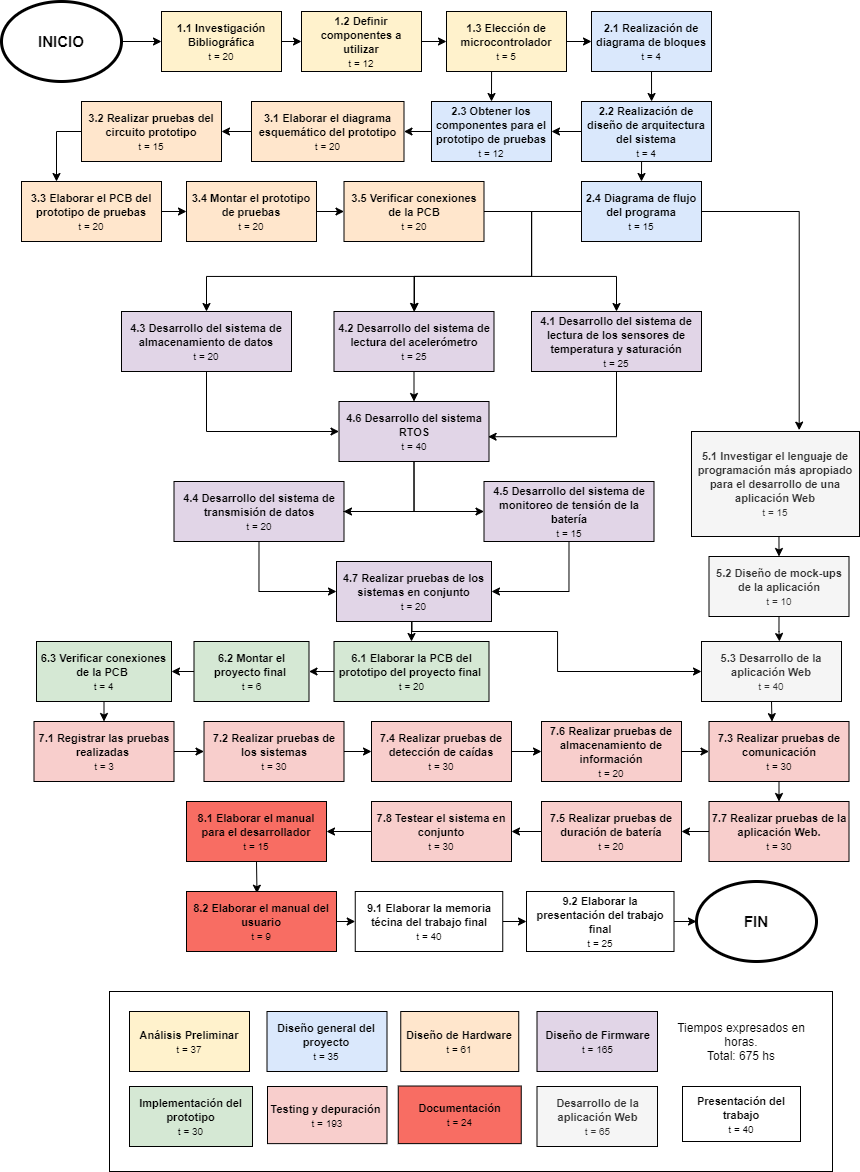
\includegraphics[width=.8\textwidth]{./Figuras/AoN.png}
\caption{Diagrama en \textit{Activity on Node}}
\label{fig:AoN}
\end{figure}

Indicar claramente en qué unidades están expresados los tiempos.
De ser necesario indicar los caminos semicríticos y analizar sus tiempos mediante un cuadro.
Es recomendable usar colores y un cuadro indicativo describiendo qué representa cada color, como se muestra en el siguiente ejemplo:



\section{8. Diagrama de Gantt}
\label{sec:gantt}

\begin{consigna}{red}
Utilizar el software Gantter for Google Drive o alguno similar para dibujar el diagrama de Gantt.

Existen muchos programas y recursos \textit{online} para hacer diagramas de gantt, entre las cuales destacamos:

\begin{itemize}
\item Planner
\item GanttProject
\item Trello + \textit{plugins}. En el siguiente link hay un tutorial oficial: \\ \url{https://blog.trello.com/es/diagrama-de-gantt-de-un-proyecto}
\item Creately, herramienta online colaborativa. \\\url{https://creately.com/diagram/example/ieb3p3ml/LaTeX}
\item Se puede hacer en latex con el paquete \textit{pgfgantt}\\ \url{http://ctan.dcc.uchile.cl/graphics/pgf/contrib/pgfgantt/pgfgantt.pdf}
\end{itemize}

Pegar acá una captura de pantalla del diagrama de Gantt, cuidando que la letra sea suficientemente grande como para ser legible. 
Si el diagrama queda demasiado ancho, se puede pegar primero la ``tabla'' del Gantt y luego pegar la parte del diagrama de barras del diagrama de Gantt.

Configurar el software para que en la parte de la tabla muestre los códigos del EDT (WBS).\\
Configurar el software para que al lado de cada barra muestre el nombre de cada tarea.\\
Revisar que la fecha de finalización coincida con lo indicado en el Acta Constitutiva.

En la figura \ref{fig:gantt}, se muestra un ejemplo de diagrama de gantt realizado con el paquete de \textit{pgfgantt}. En la plantilla pueden ver el código que lo genera y usarlo de base para construir el propio.

\begin{figure}[htbp]
\begin{center}
\begin{ganttchart}{1}{12}
  \gantttitle{2020}{12} \\
  \gantttitlelist{1,...,12}{1} \\
  \ganttgroup{Group 1}{1}{7} \\
  \ganttbar{Task 1}{1}{2} \\
  \ganttlinkedbar{Task 2}{3}{7} \ganttnewline
  \ganttmilestone{Milestone o hito}{7} \ganttnewline
  \ganttbar{Final Task}{8}{12}
  \ganttlink{elem2}{elem3}
  \ganttlink{elem3}{elem4}
\end{ganttchart}
\end{center}
\caption{Diagrama de gantt de ejemplo}
\label{fig:gantt}
\end{figure}

\end{consigna}

\section{9. Matriz de uso de recursos de materiales}
\label{sec:recursos}


\begin{table}
\label{tab:recursos}
\centering
\begin{tabularx}{\linewidth}{@{}|c|X|X|X|X|c|@{}}
\hline
\cellcolor[HTML]{C0C0C0} & \cellcolor[HTML]{C0C0C0} & \multicolumn{4}{c|}{\cellcolor[HTML]{C0C0C0}Recursos requeridos (horas)} \\ \cline{3-6} 
\multirow{-2}{*}{\cellcolor[HTML]{C0C0C0}\begin{tabular}[c]{@{}c@{}}Código\\ WBS\end{tabular}} & \multirow{-2}{*}{\cellcolor[HTML]{C0C0C0}\begin{tabular}[c]{@{}c@{}}Nombre \\ tarea\end{tabular}} & Material 1 & Material 2 & Material 3 & Material 4 \\ \hline
 &  &  &  &  &  \\ \hline
 &  &  &  &  &  \\ \hline
 &  &  &  &  &  \\ \hline
 &  &  &  &  &  \\ \hline
 &  &  &  &  &  \\ \hline
 &  &  &  &  &  \\ \hline
 &  &  &  &  &  \\ \hline
 &  &  &  &  &  \\ \hline 
 &  &  &  &  &  \\ \hline
 &  &  &  &  &  \\ \hline
 &  &  &  &  &  \\ \hline
 &  &  &  &  &  \\ \hline
 &  &  &  &  &  \\ \hline
 &  &  &  &  &  \\ \hline
 &  &  &  &  &  \\ \hline
 &  &  &  &  &  \\ \hline
 &  &  &  &  &  \\ \hline
 &  &  &  &  &  \\ \hline
 &  &  &  &  &  \\ \hline
 &  &  &  &  &  \\ \hline
 &  &  &  &  &  \\ \hline
 &  &  &  &  &  \\ \hline
 &  &  &  &  &  \\ \hline
 &  &  &  &  &  \\ \hline 
 &  &  &  &  &  \\ \hline
 &  &  &  &  &  \\ \hline
 &  &  &  &  &  \\ \hline
 &  &  &  &  &  \\ \hline

\end{tabularx}%
\end{table}


\section{10. Presupuesto detallado del proyecto}
\label{sec:presupuesto}

\begin{consigna}{red}
Si el proyecto es complejo entonces separarlo en partes:
\begin{itemize}
\item Un total global, indicando el subtotal acumulado por cada una de las áreas.
\item El desglose detallado del subtotal de cada una de las áreas.
\end{itemize}

IMPORTANTE: No olvidarse de considerar los COSTOS INDIRECTOS.

\end{consigna}

\begin{table}[htpb]
\centering
\begin{tabularx}{\linewidth}{@{}|X|c|r|r|@{}}
\hline
\rowcolor[HTML]{C0C0C0} 
\multicolumn{4}{|c|}{\cellcolor[HTML]{C0C0C0}COSTOS DIRECTOS} \\ \hline
\rowcolor[HTML]{C0C0C0} 
Descripción &
  \multicolumn{1}{c|}{\cellcolor[HTML]{C0C0C0}Cantidad} &
  \multicolumn{1}{c|}{\cellcolor[HTML]{C0C0C0}Valor unitario} &
  \multicolumn{1}{c|}{\cellcolor[HTML]{C0C0C0}Valor total} \\ \hline
 &
  \multicolumn{1}{c|}{} &
  \multicolumn{1}{c|}{} &
  \multicolumn{1}{c|}{} \\ \hline
 &
  \multicolumn{1}{c|}{} &
  \multicolumn{1}{c|}{} &
  \multicolumn{1}{c|}{} \\ \hline
\multicolumn{1}{|l|}{} &
   &
   &
   \\ \hline
\multicolumn{1}{|l|}{} &
   &
   &
   \\ \hline
\multicolumn{3}{|c|}{SUBTOTAL} &
  \multicolumn{1}{c|}{} \\ \hline
\rowcolor[HTML]{C0C0C0} 
\multicolumn{4}{|c|}{\cellcolor[HTML]{C0C0C0}COSTOS INDIRECTOS} \\ \hline
\rowcolor[HTML]{C0C0C0} 
Descripción &
  \multicolumn{1}{c|}{\cellcolor[HTML]{C0C0C0}Cantidad} &
  \multicolumn{1}{c|}{\cellcolor[HTML]{C0C0C0}Valor unitario} &
  \multicolumn{1}{c|}{\cellcolor[HTML]{C0C0C0}Valor total} \\ \hline
\multicolumn{1}{|l|}{} &
   &
   &
   \\ \hline
\multicolumn{1}{|l|}{} &
   &
   &
   \\ \hline
\multicolumn{1}{|l|}{} &
   &
   &
   \\ \hline
\multicolumn{3}{|c|}{SUBTOTAL} &
  \multicolumn{1}{c|}{} \\ \hline
\rowcolor[HTML]{C0C0C0}
\multicolumn{3}{|c|}{TOTAL} &
   \\ \hline
\end{tabularx}%
\end{table}


\section{11. Matriz de asignación de responsabilidades}
\label{sec:responsabilidades}
\begin{consigna}{red}
Establecer la matriz de asignación de responsabilidades y el manejo de la autoridad completando la siguiente tabla:

\begin{table}[htpb]
\centering
\resizebox{\textwidth}{!}{%
\begin{tabular}{|c|c|c|c|c|c|}
\hline
\rowcolor[HTML]{C0C0C0} 
\cellcolor[HTML]{C0C0C0} &
  \cellcolor[HTML]{C0C0C0} &
  \multicolumn{4}{c|}{\cellcolor[HTML]{C0C0C0}Listar todos los nombres y roles del proyecto} \\ \cline{3-6} 
\rowcolor[HTML]{C0C0C0} 
\cellcolor[HTML]{C0C0C0} &
  \cellcolor[HTML]{C0C0C0} &
  Responsable &
  Orientador &
  Equipo &
  Cliente \\ \cline{3-6} 
\rowcolor[HTML]{C0C0C0} 
\multirow{-3}{*}{\cellcolor[HTML]{C0C0C0}\begin{tabular}[c]{@{}c@{}}Código\\ WBS\end{tabular}} &
  \multirow{-3}{*}{\cellcolor[HTML]{C0C0C0}Nombre de la tarea} &
  \authorname &
  \supname &
  Nombre de alguien &
  \clientename \\ \hline
 &  &  &  &  &  \\ \hline
 &  &  &  &  &  \\ \hline
 &  &  &  &  &  \\ \hline
\end{tabular}%
}
\end{table}

{\footnotesize
Referencias:
\begin{itemize}
	\item P = Responsabilidad Primaria
	\item S = Responsabilidad Secundaria
	\item A = Aprobación
	\item I = Informado
	\item C = Consultado
\end{itemize}
} %footnotesize

Una de las columnas debe ser para el Director, ya que se supone que participará en el proyecto.
A su vez se debe cuidar que no queden muchas tareas seguidas sin ``A'' o ``I''.

Importante: es redundante poner ``I/A'' o ``I/C'', porque para aprobarlo o responder consultas primero la persona debe ser informada.

\end{consigna}

\section{12. Gestión de riesgos}
\label{sec:riesgos}

\begin{consigna}{red}
a) Identificación de los riesgos (al menos cinco) y estimación de sus consecuencias:
 
Riesgo 1: detallar el riesgo (riesgo es algo que si ocurre altera los planes previstos)
\begin{itemize}
\item Severidad (S): mientras más severo, más alto es el número (usar números del 1 al 10).\\
Justificar el motivo por el cual se asigna determinado número de severidad (S).
\item Probabilidad de ocurrencia (O): mientras más probable, más alto es el número (usar del 1 al 10).\\
Justificar el motivo por el cual se asigna determinado número de (O). 
\end{itemize}   

Riesgo 2:
\begin{itemize}
\item Severidad (S): 
\item Ocurrencia (O):
\end{itemize}

Riesgo 3:
\begin{itemize}
\item Severidad (S): 
\item Ocurrencia (O):
\end{itemize}


b) Tabla de gestión de riesgos:      (El RPN se calcula como RPN=SxO)

\begin{table}[htpb]
\centering
\begin{tabularx}{\linewidth}{@{}|X|c|c|c|c|c|c|@{}}
\hline
\rowcolor[HTML]{C0C0C0} 
Riesgo & S & O & RPN & S* & O* & RPN* \\ \hline
       &   &   &     &    &    &      \\ \hline
       &   &   &     &    &    &      \\ \hline
       &   &   &     &    &    &      \\ \hline
       &   &   &     &    &    &      \\ \hline
       &   &   &     &    &    &      \\ \hline
\end{tabularx}%
\end{table}

Criterio adoptado: 
Se tomarán medidas de mitigación en los riesgos cuyos números de RPN sean mayores a...

Nota: los valores marcados con (*) en la tabla corresponden luego de haber aplicado la mitigación.

c) Plan de mitigación de los riesgos que originalmente excedían el RPN máximo establecido:
 
Riesgo 1: plan de mitigación (si por el RPN fuera necesario elaborar un plan de mitigación).
  Nueva asignación de S y O, con su respectiva justificación:
  - Severidad (S): mientras más severo, más alto es el número (usar números del 1 al 10).
          Justificar el motivo por el cual se asigna determinado número de severidad (S).
  - Probabilidad de ocurrencia (O): mientras más probable, más alto es el número (usar del 1 al 10).
          Justificar el motivo por el cual se asigna determinado número de (O).

Riesgo 2: plan de mitigación (si por el RPN fuera necesario elaborar un plan de mitigación).
 
Riesgo 3: plan de mitigación (si por el RPN fuera necesario elaborar un plan de mitigación).

\end{consigna}


\section{13. Gestión de la calidad}
\label{sec:calidad}

\begin{consigna}{red}
Para cada uno de los requerimientos del proyecto indique:
\begin{itemize} 
\item Req \#1: copiar acá el requerimiento.

Verificación y validación:

\begin{itemize}
\item Verificación para confirmar si se cumplió con lo requerido antes de mostrar el sistema al cliente. Detallar 
\item Validación con el cliente para confirmar que está de acuerdo en que se cumplió con lo requerido. Detallar  
\end{itemize}

\end{itemize}

Tener en cuenta que en este contexto se pueden mencionar simulaciones, cálculos, revisión de hojas de datos, consulta con expertos, mediciones, etc.

\end{consigna}

\section{14. Comunicación del proyecto}
\label{sec:comunicaciones}

El plan de comunicación del proyecto es el siguiente:

\begin{table}[htpb]
\centering
\begin{tabularx}{\linewidth}{@{}|X|C{2.4cm}|C{3cm}|C{1.8cm}|C{2cm}|C{2.1cm}|@{}}
\hline
\rowcolor[HTML]{C0C0C0} 
\multicolumn{6}{|c|}{\cellcolor[HTML]{C0C0C0}PLAN DE COMUNICACIÓN DEL PROYECTO}           \\ \hline
\rowcolor[HTML]{C0C0C0} 
¿Qué comunicar? & Audiencia & Propósito & Frecuencia & Método de comunicac. & Responsable \\ \hline
                &           &           &            &                      &             \\ \hline
                &           &           &            &                      &             \\ \hline
                &           &           &            &                      &             \\ \hline
                &           &           &            &                      &             \\ \hline
                &           &           &            &                      &             \\ \hline
\end{tabularx}
\end{table}

\section{15. Gestión de compras}
\label{sec:compras}

\begin{consigna}{red}
En caso de tener que comprar elementos o contratar servicios:
a) Explique con qué criterios elegiría a un proveedor.
b) Redacte el Statement of Work correspondiente.
\end{consigna}

\section{16. Seguimiento y control}
\label{sec:seguimiento}

\begin{consigna}{red}
Para cada tarea del proyecto establecer la frecuencia y los indicadores con los se seguirá su avance y quién será el responsable de hacer dicho seguimiento y a quién debe comunicarse la situación (en concordancia con el Plan de Comunicación del proyecto).

El indicador de avance tiene que ser algo medible, mejor incluso si se puede medir en \% de avance. Por ejemplo,se pueden indicar en esta columna cosas como ``cantidad de conexiones ruteadeas'' o ``cantidad de funciones implementadas'', pero no algo genérico y ambiguo como ``\%'', porque el lector no sabe porcentaje de qué cosa.

\end{consigna}

\begin{longtable}{|m{1cm}|m{3.5cm}|m{2.2cm}|m{2cm}|m{3cm}|m{1.5cm}|}
\hline
\rowcolor[HTML]{C0C0C0} 
\multicolumn{6}{|c|}{\cellcolor[HTML]{C0C0C0}SEGUIMIENTO DE AVANCE}                                                                       \\ \hline
\rowcolor[HTML]{C0C0C0} 
Tarea del WBS 			& Indicador de avance & Frecuencia de reporte & Resp. de seguimiento & Persona a ser informada & Método de comunic. \\ \hline
\endfirsthead

\hline
\rowcolor[HTML]{C0C0C0} 
\multicolumn{6}{c}{\cellcolor[HTML]{C0C0C0}SEGUIMIENTO DE AVANCE}                                                                       \\ \hline
\rowcolor[HTML]{C0C0C0} 
Tarea del WBS 			& Indicador de avance & Frecuencia de reporte & Resp. de seguimiento & Persona a ser informada & Método de comunic. \\ \hline
\endhead

\multicolumn{6}{c}{Continúa}
\endfoot

\endlastfoot

1.1	& Fecha de inicio  & Única vez al comienzo & \authorname & \clientename, \supname & email \\ \hline
2.1	& Avance de las subtareas  & Mensual mientras dure la tarea & \authorname & \clientename, \supname & email \\ \hline

\end{longtable}

\begin{table}[!htpb]
\centering
%\begin{tabularx}{\linewidth}{@{}|X|X|X|X|X|X|@{}}
\begin{tabularx}{\linewidth}{@{}|X|C{2.5cm}|C{3cm}|C{2cm}|C{2cm}|C{2.5cm}|@{}}
\hline
\rowcolor[HTML]{C0C0C0} 
\multicolumn{6}{|c|}{\cellcolor[HTML]{C0C0C0}SEGUIMIENTO DE AVANCE}                                                                       \\ \hline
\rowcolor[HTML]{C0C0C0} 
Tarea del WBS & Indicador de avance & Frecuencia de reporte & Resp. de seguimiento & Persona a ser informada & Método de comunic. \\ \hline
 &  &  &  &  &  \\ \hline
 &  &  &  &  &  \\ \hline
 &  &  &  &  &  \\ \hline
 &  &  &  &  &  \\ \hline
 &  &  &  &  &  \\ \hline
\end{tabularx}%
%}
\end{table}

\section{17. Procesos de cierre}    
\label{sec:cierre}

\begin{consigna}{red}
Establecer las pautas de trabajo para realizar una reunión final de evaluación del proyecto, tal que contemple las siguientes actividades:

\begin{itemize}
\item Pautas de trabajo que se seguirán para analizar si se respetó el Plan de Proyecto original:
 - Indicar quién se ocupará de hacer esto y cuál será el procedimiento a aplicar. 
\item Identificación de las técnicas y procedimientos útiles e inútiles que se utilizaron, y los problemas que surgieron y cómo se solucionaron:
 - Indicar quién se ocupará de hacer esto y cuál será el procedimiento para dejar registro.
\item Indicar quién organizará el acto de agradecimiento a todos los interesados, y en especial al equipo de trabajo y colaboradores:
  - Indicar esto y quién financiará los gastos correspondientes.
\end{itemize}

\end{consigna}


\end{document}
